\documentclass{article}\usepackage[]{graphicx}\usepackage[]{color}
% maxwidth is the original width if it is less than linewidth
% otherwise use linewidth (to make sure the graphics do not exceed the margin)
\makeatletter
\def\maxwidth{ %
  \ifdim\Gin@nat@width>\linewidth
    \linewidth
  \else
    \Gin@nat@width
  \fi
}
\makeatother

\definecolor{fgcolor}{rgb}{0.345, 0.345, 0.345}
\newcommand{\hlnum}[1]{\textcolor[rgb]{0.686,0.059,0.569}{#1}}%
\newcommand{\hlstr}[1]{\textcolor[rgb]{0.192,0.494,0.8}{#1}}%
\newcommand{\hlcom}[1]{\textcolor[rgb]{0.678,0.584,0.686}{\textit{#1}}}%
\newcommand{\hlopt}[1]{\textcolor[rgb]{0,0,0}{#1}}%
\newcommand{\hlstd}[1]{\textcolor[rgb]{0.345,0.345,0.345}{#1}}%
\newcommand{\hlkwa}[1]{\textcolor[rgb]{0.161,0.373,0.58}{\textbf{#1}}}%
\newcommand{\hlkwb}[1]{\textcolor[rgb]{0.69,0.353,0.396}{#1}}%
\newcommand{\hlkwc}[1]{\textcolor[rgb]{0.333,0.667,0.333}{#1}}%
\newcommand{\hlkwd}[1]{\textcolor[rgb]{0.737,0.353,0.396}{\textbf{#1}}}%
\let\hlipl\hlkwb

\usepackage{framed}
\makeatletter
\newenvironment{kframe}{%
 \def\at@end@of@kframe{}%
 \ifinner\ifhmode%
  \def\at@end@of@kframe{\end{minipage}}%
  \begin{minipage}{\columnwidth}%
 \fi\fi%
 \def\FrameCommand##1{\hskip\@totalleftmargin \hskip-\fboxsep
 \colorbox{shadecolor}{##1}\hskip-\fboxsep
     % There is no \\@totalrightmargin, so:
     \hskip-\linewidth \hskip-\@totalleftmargin \hskip\columnwidth}%
 \MakeFramed {\advance\hsize-\width
   \@totalleftmargin\z@ \linewidth\hsize
   \@setminipage}}%
 {\par\unskip\endMakeFramed%
 \at@end@of@kframe}
\makeatother

\definecolor{shadecolor}{rgb}{.97, .97, .97}
\definecolor{messagecolor}{rgb}{0, 0, 0}
\definecolor{warningcolor}{rgb}{1, 0, 1}
\definecolor{errorcolor}{rgb}{1, 0, 0}
\newenvironment{knitrout}{}{} % an empty environment to be redefined in TeX

\usepackage{alltt}
\usepackage{Sweave}
\usepackage{float}
\usepackage{graphicx}
\usepackage{tabularx}
\usepackage{hyperref}
\usepackage{siunitx}
\usepackage{amssymb} % for math symbols
\usepackage{amsmath} % for aligning equations
\usepackage{textcomp}
\usepackage{mdframed}
\usepackage{natbib}
\bibliographystyle{..//references/styles/besjournals.bst}
\usepackage[small]{caption}
\setlength{\captionmargin}{30pt}
\setlength{\abovecaptionskip}{0pt}
\setlength{\belowcaptionskip}{10pt}
\topmargin -1.5cm        
\oddsidemargin -0.04cm   
\evensidemargin -0.04cm
\textwidth 16.59cm
\textheight 21.94cm 
%\pagestyle{empty} %comment if want page numbers
\parskip 7.2pt
\renewcommand{\baselinestretch}{1.5}
\parindent 0pt
%\usepackage{lineno}
%\linenumbers

%cross referencing:
\usepackage{xr}
\externaldocument{chillfrz_supp}

\newmdenv[
  topline=true,
  bottomline=true,
  skipabove=\topsep,
  skipbelow=\topsep
]{siderules}

%% R Script


\IfFileExists{upquote.sty}{\usepackage{upquote}}{}
\begin{document}

\noindent \textbf{\Large{False spring damage on temperate tree seedlings is amplified with winter warming}}

\noindent Authors:\\
C. J. Chamberlain $^{1,2}$, K. Woodruff $^{1}$ \& E. M. Wolkovich $^{1,2,3}$
\vspace{2ex}\\
\emph{Author affiliations:}\\
$^{1}$Arnold Arboretum of Harvard University, 1300 Centre Street, Boston, Massachusetts, USA; \\
$^{2}$Organismic \& Evolutionary Biology, Harvard University, 26 Oxford Street, Cambridge, Massachusetts, USA; \\
$^{3}$Forest \& Conservation Sciences, Faculty of Forestry, University of British Columbia, 2424 Main Mall, Vancouver, BC V6T 1Z4\\
\vspace{2ex}
$^*$Corresponding author: 248.953.0189; cchamberlain@g.harvard.edu\\

\renewcommand{\thetable}{\arabic{table}}
\renewcommand{\thefigure}{\arabic{figure}}
\renewcommand{\labelitemi}{$-$}
\setkeys{Gin}{width=0.8\textwidth}

%%%%%%%%%%%%%%%%%%%%%%%%%%%%%%%%%%%%%%%%%%%%%%%
%%%%%%%%%%%%%%%%%%%%%%%%%%%%%%%%%%%%%%%%%%%%%%%


\section*{Introduction}
% emw-midApril2020: When do you write this up, be careful not to plagiarize yourself. The text needs to be different enough from your other papers (I fin that this can be really hard in methods, but should be do-able in the rest of the text)
\begin{enumerate}
\item The timing of spring in temperate deciduous forests shapes plant and animal communities and influences ecosystem services from agriculture to carbon sequestration to forest management. 
  \begin{enumerate} 
  \item With warming temperatures in the Northern Hemisphere, spring phenology (i.e., budburst and leafout) is advancing.
  \item As budburst and leafout are strongly cued by temperature, species' ranges and growing season lengths are highly susceptible to change with climate-induced warming \citep{Chuine2001}. 
  \item These advancements in spring phenology is leading to increased carbon uptake across temperate forests, which are essential carbon sinks that combat the negative effects of climate change \citep{Keenan2014}.
  \end{enumerate}
  
\item And though the Northern Hemisphere is getting warmer, climate change is affecting general temperature trends but extreme weather events (e.g., polar vortexes) are still occurring. 
  \begin{enumerate}
  \item These weather events can in turn have big impacts on plant development each spring. 
  \item One such event is known as a `false spring', which is when temperatures drop below freezing \citep[][i.e., below -2.2$^{\circ}$C]{Schwartz2002} after budburst has initiated.
  \item During budburst, it is a risky time for plants \citep{Chamberlain2019} and plants can sustain major damage if a freeze hits during this time. 
  \item It has been reported that it can take up to 16-38 days for plants to refoliate after leaf loss from a false spring \citep{Augspurger2009, Augspurger2013, Gu2008, Menzel2015}. 
  \item Such damage can have cascading effects to pollinators \citep{Boggs2012, Pardee2017}, nutrient cycling and carbon uptake as well as forest recruitment \citep{Hufkens2012, Klosterman2018, Richardson2013}
  \item Further, if a false spring occurs and damages a plant, that plant is at an increased risk of experiencing an additional false spring as freezing temperatures can slow the rate of budburst \citep{Augspurger2009} resulting in even greater reprecussions for the ecosystem.
  \item False springs are predicted to increase in certain regions as climate change progresses, thus understanding the impacts of false springs on forests is essential for forest management strategies and climate forecasting \citep{OBrien2019}.
  \end{enumerate}
  
\item False springs are not the only things that may complicate forecasts.
  \begin{enumerate}
  \item Winters are warming, which could potentially impact not only phenology but also growth.
  \item Warmer winters directly impact one of the three major cues plants use to time budburst: (1) over-winter cold temperatures (chilling), (2) warming spring temperatures (forcing) and (3) longer daylengths (photoperiod).
  \item Due to harsh winters and unpredictable springs, temperate tree and shrub species have evolved to use a two-phase sequence of dormancy.
  \item The first phase---endodormancy---is the period of winter when temperate trees are inhibited from growing, regardless of the outdoor environment and individuals require a certain number of chilling hours to exit this initial phase \citep{Charrier2011}.
  \item The sceond phase---ecodormancy---begins after the chilling requirement has been met and is the period of time when growth can occur but the external environment is not conducive to growth (e.g. too cold) \citep{Basler2012}. 
  \item With endo- and ecodormancy phases, temperate plants are better protected against stochastic warm spells in the winter and reduce the risk of a false spring \citep{Basler2014} but climate change complicates the timing and depth of dormancy \citep{Charrier2011}.
  \end{enumerate}

\item Winter warming and its effect on dormancy could impact the quality of budburst \citep{Cleland2007,Bonhomme2010}. 
  \begin{enumerate}
  \item Decreases in chilling temperatures from climate change could affect budburst timing \citep{Nanninga2017}, as well as the synchrony of budburst within a population or even within an individual \citep{Sanzperez2009}.
  \item And, reduced chilling---especially if there are fewer cold nights with warming---could impact a plant's tolerance of freezing temperatures throughout the winter \citep{Charrier2011}.
  \item With decreased freezing tolerance, plants are susceptible to damage to leaf tissue, canopy dieback, xylem embolism and injury to the shoot apical meristem, all of which could greatly reduce a plant's ability to recover for the remainder of the growing season or even survive until the next season \citep{Sakai1987,Gu2008}.
  \item Thus, understanding the interplay of warming winters and false spring risk is critical for understanding how temperate forests will change in the future. 
  \end{enumerate}
  
\item Temperate tree and shrub species respond to the three phenological cues in varying ways to reach budburst.
  \begin{enumerate} % emw-midApril2020: I pulled these points from above as they seemed to specific for how early they were in the intro. I think they could work -- with additional info -- to set up that species are not all the same. From just above the intro could flow: An ideal strategy might thus be to require high chilling, leafout late and avoid frost, but competition between plants puts pressure on individuals to leafout as early as possible and gain priority access to resources ... Thus plants have multiple strategies -- some are late (avoidance), some avoid by speeding through the risky bit (add your info on freezing tolerance), some may try to tolerate .... Then perhaps another paragraph on differences across functional groups and species.
  \item Ideally, individuals would evolve to require high levels of chilling to delay budburst and ultimately diminish false spring risk but competition for nutrients, water and light resources in the early spring pushes individuals to leafout earlier.
  \item Plants use myriad strategies to minimize false spring risk but maximize growth.
  \item As freezing tolerance in a plant steadily decreases after budburst begins until the leaf is fully unfolded \citep{Lenz2016}, some species avoid false spring risk by employing mechanisms to speed through this high risk timeframe.
  \item Other species use trichomes or high solute concentrations in the leaves to increase freezing tolerance during budburst \citep{Agrawal2004, Sakai1987}, while still other species have high chilling, forcing and/or photoperiod requirements and leafout late in the spring to avoid damage from false springs altogether.
  \end{enumerate}
  
\item Young trees and understory species generally initiate budburst before the canopy trees to benefit from higher light levels \citep {Augspurger2008, Vitasse2013}, which potentially puts these species and individuals at higher risk of freeze damage \citep{Vitasse2014}.
  \begin{enumerate}
  \item Species typically leafout in a similar sequence, with understory species leafing out earlier and higher canopy trees leafing out last but many studies are predicting substantial shifts in chronological order and reassembly of species' leafout with climate change \citep{Roberts2015, Laube2014}.
  \item As warming alters winter temperatures and false spring prevalence, phenological cues and their interactions are anticipated to change, which could greatly alter competition among forest species for early season resources and ultimately impact species diversity and carbon uptake in temperate forests.
  \end{enumerate}
  
\item Here, we assessed the effects of over-winter chilling length and false springs on seedling phenology and growth across eight temperate tree and shrub species. 
  \begin{enumerate}
  \item Individuals were exposed to three levels of over-winter chilling. 
  \item Once budburst was initiated, half of the individuals were exposed to freezing temperatures at -3$^{\circ}$C to mimic a false spring event. 
  \item Individuals were then put in a greenhouse for the remainder of the growing season to ask: (1) How does the accumulation of over-winter chilling hours and (2) how do false spring events impact phenology, physical leaf characteristics and growth?
  \end{enumerate}
\end{enumerate}
  

\section*{Methods}
\subsection*{Plant Selection and Material}
\begin{enumerate}
\item We chose 10 temperate woody plant tree and shrub species with varying phenologies, that were not used as crops or ornamental species: \textit{Acer saccharinum} L., \textit{Alnus incana rugosa} L., \textit{Betula papyrifera} Marsh., \textit{Betula populifolia} Marsh., \textit{Cornus racemosa} Lam., \textit{Fagus grandifolia} Ehrh., \textit{Nyssa sylvatica} Marsh., \textit{Salix purpurea} L., \textit{Sorbus americana} Marsh., and \textit{Viburnum dentatum} L.
  \begin{enumerate}
  \item We received 48 dormant bare root seedlings---each measuring 6-12 inches---for each species from Cold Stream Farm LLC (Freesoil, MI; 44$^{\circ}$6' N -86$^{\circ}$12' W) for a total of 480 individuals.
  \item Upon receipt, plants were potted in POT INFO AND SOIL INFO HERE!! and placed in growth chambers at the Weld Hill Research Building of the Arnold Arboretum (Boston, MA; 42$^{\circ}$17' N -71$^{\circ}$8' W) at 4$^{\circ}$C to maintain dormancy.
  \item Two species---\textit{Fagus grandifolia} and \textit{Nyssa sylvatica}---were delivered as root cuttings rather than seedlings and had to be removed from the experiment resulting in eight total species and 384 individuals.
  \item After all individuals had leafed out, all seedlings were up-potted to new pots (NEW POT SIZE HERE) and given fertilizer (FERTILIZER INFO HERE).
  \end{enumerate}
\end{enumerate}
\subsection*{Growth Chamber and Greenhouse Conditions}
\begin{enumerate}
\item Individuals were randomly selected and placed in six experimental treatments: 4 weeks of chilling at 4$^{\circ}$C x no false spring, 4 weeks of chilling at 4$^{\circ}$C x false spring, 6 weeks of chilling at 4$^{\circ}$C x no false spring, 6 weeks of chilling at 4$^{\circ}$C x false spring,
8 weeks of chilling at 4$^{\circ}$C x no false spring, 8 weeks of chilling at 4$^{\circ}$C x false spring.
  \begin{enumerate}
  \item While individuals were in the growth chamber under chilling conditions, photoperiod was mantained at eight hour days.
  \item Lighting within the chambers was provided through a combination of T5HO fluorescent lamps with halogen incandescent bulbs at roughly 250 $\mu mol/m^{2}/s$.
  \item Individuals were rotated within and among growth chambers every two weeks to eliminate possible growth chamber effects.
  \end{enumerate}
\item Once chilling was completed, individuals were moved to a greenhouse with mean daytime temperature of 15$^{\circ}$C and a mean nighttime temperature of 10$^{\circ}$C.
  \begin{enumerate}
  \item Photoperiod was set to 12 hour days throughout the spring until all individuals reached full leaf expansion.
  \item After all individuals reached full leaf expansion, greenhouse temperatures and photoperiods were kept ambient (see Supplemental Materials for more information). 
  \end{enumerate}
\end{enumerate}
\subsection*{Phenology and False Spring Treatment}
\begin{enumerate}
\item Phenology observations were taken every 2-3 days through full leaf expansion and then recorded weekly over the summer.
  \begin{enumerate}
  \item Budburst was denoted as BBCH stage 07, which is `beginning of sprouting or bud breaking' and monitored until full leaf expansion (BBCH stage 19) in order to evaluate the duration of vegetative risk for each individual \citep{Finn2007}.
  \item For the individuals under the `false spring treatment', once at least 50\% of the buds were at BBCH stage 07 but the individual had not yet reached BBCH stage 19, they were placed in a growth chamber set to mimic a false spring event.
  \item Individuals receiving the false spring treatment were placed in a growth chamber for 14 hours, starting at 6pm. 
  \item Temperatures in the growth chamber were ramped down: 6pm to 10$^{\circ}$C, 8pm to 5$^{\circ}$C, 10pm to 0$^{\circ}$C, 12am to -3$^{\circ}$C, 3am to 0$^{\circ}$C, 4am to 5$^{\circ}$C, 6am to 10$^{\circ}$C and 8am temperatures rose again to 15$^{\circ}$C (Figure \ref{fig:gccond}).
  \item After 8am the following day, individuals were collected at placed back in the greenhouse with all of the other plants. 
  \item Once all individuals reached full leaf expansion (BBCH stage 19), phenology observations were made weekly until August 1st, when observations were made every 2-3 days again to monitor fall phenology. 
  \item Individuals were monitored until complete budset, at which point they were harvested for biomass measurements.
  \end{enumerate}
\end{enumerate}
\subsection*{Growth measurements}
\begin{enumerate}
\item Growth was closely measured throughout the entirety of the experiment. 
  \begin{enumerate}
  \item Height was measured three times throughout the growing season: the day an individual reached full leaf expansion, 60 days after full leaf out and when an individual reached complete budset. 
  \item We measured the chlorophyll content of four leaves on each individual 60 days after full leaf out using an atLEAF CHL PLUS Chlorophyll meter (\url{https://www.atleaf.com/atLEAF\_CHL\_PLUS}).
  \item The average chlorophyll content was calculated and then converted to mg/cm\textsuperscript{2} using the atLEAF CHL PLUS conversion tool (\url{https://www.atleaf.com/SPAD}).
  \item We measured leaf thickness using a Shars Digital Micrometer (\url{https://www.shars.com/products\linebreak/measuring/micrometers/0-1-solid-metal-frame-electronic-outside-micrometer}) and leaf toughness in Newtons using a Shimpo Digital Force Gauge (\url{http://shimpoinstruments.com/force\_gauges/fg-3000}) on two leaves for each individual.
  \item Additionally, we monitored damage to the shoot apical meristem, which consisted of complete damage or disruption of growth in the main stem and resulted in early dormancy induction or reliance on lateral shoot growth.
  \item Finally, belowground and aboveground biomass were harvested after an individual reached complete budset to include leaves in our biomass calculations. 
  \item Belowground and aboveground plant material were separated and then put in a Shel Lab Forced Air Oven (\url{https://www.sheldonmanufacturing.com/shel\-lab\-products/productid/SMO28HP\-2}) at 60$^{\circ}$C for at least 4 days. 
  \end{enumerate}
\end{enumerate}
\subsection*{Data analysis}
\begin{enumerate}
\item Using Bayesian hierarchical models with the brms package \citep{brms}, version 2.3.1,  in R \citep{R}, version 3.3.1, we estimate the effects of chilling duration, false spring treatment and all two-way interactions as predictors on: (1) duration of vegetative risk, (2) growing season length, (3) total growth in centimeters, (4) chlorophyll content, (5) leaf thickness, (6) leaf toughness, (7) shoot apical meristem damage and (8) total biomass. % CUT FOR NOW: and (9) belowground to aboveground biomass ratio. 
  \begin{enumerate} %emw-midApril2020: I would move all equations to the supp as your methods are long already and they are fairly standard equations
  \item Species are modeled hierarchically as grouping factors, which generates an estimate and posterior distribution of the overall response across the eight species used in our experiment.
  \item We ran four chains, each with 2 500 warm-up iterations and 4 000 sampling iterations for a total of 6 000 posterior samples for each predictor for each model using weakly informative priors. 
  \item Increasing priors three-fold did not impact our results.
  \item We evaluated our model performance based on $\hat{R}$ values that were close to one and did not include models with divergent transitions in our results. 
  \item We also evaluated high $n_{eff}$ (4000 for most parameters, but as low as 1400 for a couple of parameters in the shoot apical meristem model). 
  \item We additionally assessed chain convergence and posterior predictive checks visually \citep{BDA}.
  \end{enumerate}
\end{enumerate}

\section*{Results}
\begin{enumerate}
\item False springs and chilling durations impacted individual phenology but not phenological rank within the community. 
  \begin{enumerate}
  \item Order of leafout timing was consistent across all treatments, with \textit{Salix purpurea} always being first to leafout, followed by \textit{Betula papyrifera}, \textit{B. populifolia} and \textit{Cornus racemosa} and finally by \textit{Alnus rugosa}, \textit{Sorbus americana}, \textit{Viburnum dentatum} and \textit{Acer saccharinum} (Figure \ref{fig:rank}).
  \item \textit{Viburnum dentatum} was the only species to change rank across treatments, though it consistently was grouped with the later-leafout group of species.
  \item Order of budset timing was also consistent across all treatments, with \textit{Cornus racemosa} and \textit{Sorbus americana} being first to set bud, followed by \textit{Betula papyrifera} and \textit{Acer saccharinum} and finally by \textit{Viburnum dentatum}, \textit{B. populifolia}, \textit{Salix purpurea} and \textit{Alnus rugosa} (Figure \ref{fig:bsetrank}).
  \item \textit{Acer saccharinum} was the only species to change rank across treatments, though it consistently was grouped with \textit{Betula papyrifera} and \textit{Viburnum dentatum}.
  \item Individuals exposed to the false spring treatment had longer durations of vegetative risk for both the four weeks and six weeks of chilling cohorts (2.97 $\pm$ 0.79 and 1.53 $\pm$ 1.14, respectively) Figure \ref{fig:muphen}a) and Table \ref{tab:suppmoddvr}).
  \item Longer chilling treatments reduced the duration of vegetative risk, especially in the 8 weeks of chilling cohort (-2.67 $\pm$ 1.14), Figure \ref{fig:muphen}a) and Table \ref{tab:suppmoddvr}).
  \item Additionally, individuals that received eight weeks of chilling did not experience major changes in their durations of vegetative risk (0.92 $\pm$ 1.08), Figure \ref{fig:muphen}a and Table \ref{tab:suppmoddvr}). 
  \item With increases in chilling duration, the growing season length decreased for individuals exposed to six and eight weeks of chilling (2.48 $\pm$ 4.87 for six weeks and -9.66 $\pm$ 5 for eight weeks), Figure \ref{fig:muphen}b) and Table \ref{tab:suppmodgs}).
  \end{enumerate}
  
\item False springs affected physical leaf traits.
  \begin{enumerate}
  \item Leaf chlorophyll content decreased under false spring conditions, especially in the six weeks (-1.45 $\pm$ 1.16) and eight weeks (-2.03 $\pm$ 1.07) Figure \ref{fig:muchl}) and Table \ref{tab:suppmodchl}) of chilling cohorts.
  \item Leaf toughness decreased across all chilling treatments under false spring conditions (-0.05 $\pm$ 0.02 for four weeks of chilling, -0.09 $\pm$ 0.03 for six weeks of chilling and -0.08 $\pm$ 0.03 for eight weeks of chilling), Figure \ref{fig:muleaf}a) and Table \ref{tab:suppmodtough}).
  \item Additionally, leaf thickness decreased across all chilling treatments under false spring conditions (-8.9 $\pm$ 3.74 for four weeks of chilling, -3.5 $\pm$ 5.31 for six weeks of chilling and -15.78 $\pm$ 5.25 for eight weeks of chilling), Figure \ref{fig:muleaf}b) and Table \ref{tab:suppmodthick}).
  \end{enumerate}
  
\item False springs impacted growth.
  \begin{enumerate}
  \item Across all chilling treatments, individuals exposed to false springs experienced more damage to the shoot apical meristem (2.07 $\pm$ 0.97 for four weeks, 1.33 $\pm$ 1.42 for six weeks and 2.17 $\pm$ 1.31 for eight weeks), Figure \ref{fig:mugrowth}a) and Table \ref{tab:suppmodmeri}) 
  \item Shoot growth over the growing season increased with increased chilling durations (2.92 $\pm$ 4.14 for six weeks of chilling and 11 $\pm$ 4.01 for eight weeks of chilling) except growth was not affected under false spring conditions (-0.42 $\pm$ 6.37 for six weeks and 4.73 $\pm$ 5.49 for eight weeks), Figure \ref{fig:muheight}) and Table \ref{tab:suppmodht})).
  \item Individuals exposed to false spring conditions had lower total biomasses when they were exposed to only four weeks of chilling (-3.45 $\pm$ 2.78) but there was very little change in total biomass under false spring conditions compared to the control for both the six weeks of chilling cohort (-3.62 $\pm$ 4.04) and the eight weeks of chilling cohort (2.88 $\pm$ 3.04), Figure \ref{fig:mugrowth}b) and Table \ref{tab:suppmodtotbio})).
  \end{enumerate}
\end{enumerate}

\section*{Discussion}
\begin{enumerate}
\item Growth chamber studies and climate model projections predict substantial shifts in species leafout order under climate change conditions \citep{Roberts2015, Laube2014}, other studies using long-term phenology observations suggest leafout phenology order is consistent across years \citep{Wesolowski2006}.
  \begin{enumerate}{
  \item We are not seeing major shifts in species leafout order except for in \textit{Viburnum dentatum}, which still leafs out within the later cohort of species across all treatments.
  \item Therefore, we do not predict major reassembly of forest communities due to winter warming or false spring incidence. 
  \end{enumerate}

\item Chilling length greatly influences spring phenology and can compensate for the detrimental effects of false springs.
  \begin{enumerate}
  \item False springs increase the duration of vegetive risk, leading to an increased risk in multiple false spring risks in one season.
  \item But chilling can compensate for this increase in duration of vegetative risk: if the chilling requirement is met, the rate of budburst does not increase with a false spring event.
  \item This suggests chilling is more important for seedlings in terms of exposure to multiple false springs.
  \item With climate change and warming temperatures, over-winter chilling is anticipated to decrease and false springs are predicted to increase in certain regions.
  \item This combination could greatly impact plant performance, survival and shape species distributions, ultimately affecting crucial processes such as carbon uptake and nutrient cycling.
  \end{enumerate}
  
\item False springs greatly impact the physical characteristics of the leaf.
  \begin{enumerate}
  \item With chlorophyll content, leaf toughness and leaf thickness decreasing, the quality of the leaf dwindles.
  \item This reduction in quality could subsequently lead to an increase in herbivory risk \citep{Onda2011}.
  \item Further studies that assess the secondary compounds and total phenolic content \citep{Ayres1993, Webber2016} of the leaves exposed to false springs are needed to better understand the level of herbivory risk. 
  \end{enumerate}
  
\item With sufficient chilling, false springs are less damaging to seedling growth.
  \begin{enumerate}
  \item However, false springs consistently impair shoot apical meristem growth, which can lead to relience on lateral shoot growth, rendering inefficient growth patterns.
  \item Shoot apical meristem damage---if significant within a stand---can lead to declines in recruitment \citep{Rhodes2018}. 
  \end{enumerate}
  
\item Understanding the impacts of false springs coupled with reduced over-winter chilling is essential for forecasting.
  \begin{enumerate}
  \item Our findings have large implications for forest recruitment.
  \item With over-winter chilling decreasing with climate change, seedlings are more at risk of sustaining damage from false spring events. 
  \item Understanding recruitment and inter- and intraspecific competition with false springs is crucial. 
  \item If individuals that initiate budburst earlier are more at risk of false spring exposure, this could lead to dieback of early-budbursting species in temperate forests with climate change.
  \end{enumerate}
\end{enumerate}




\bibliography{..//references/chillfreeze.bib}

\section*{Tables and Figures}
  {\begin{figure} [H]
  -\begin{center}
  -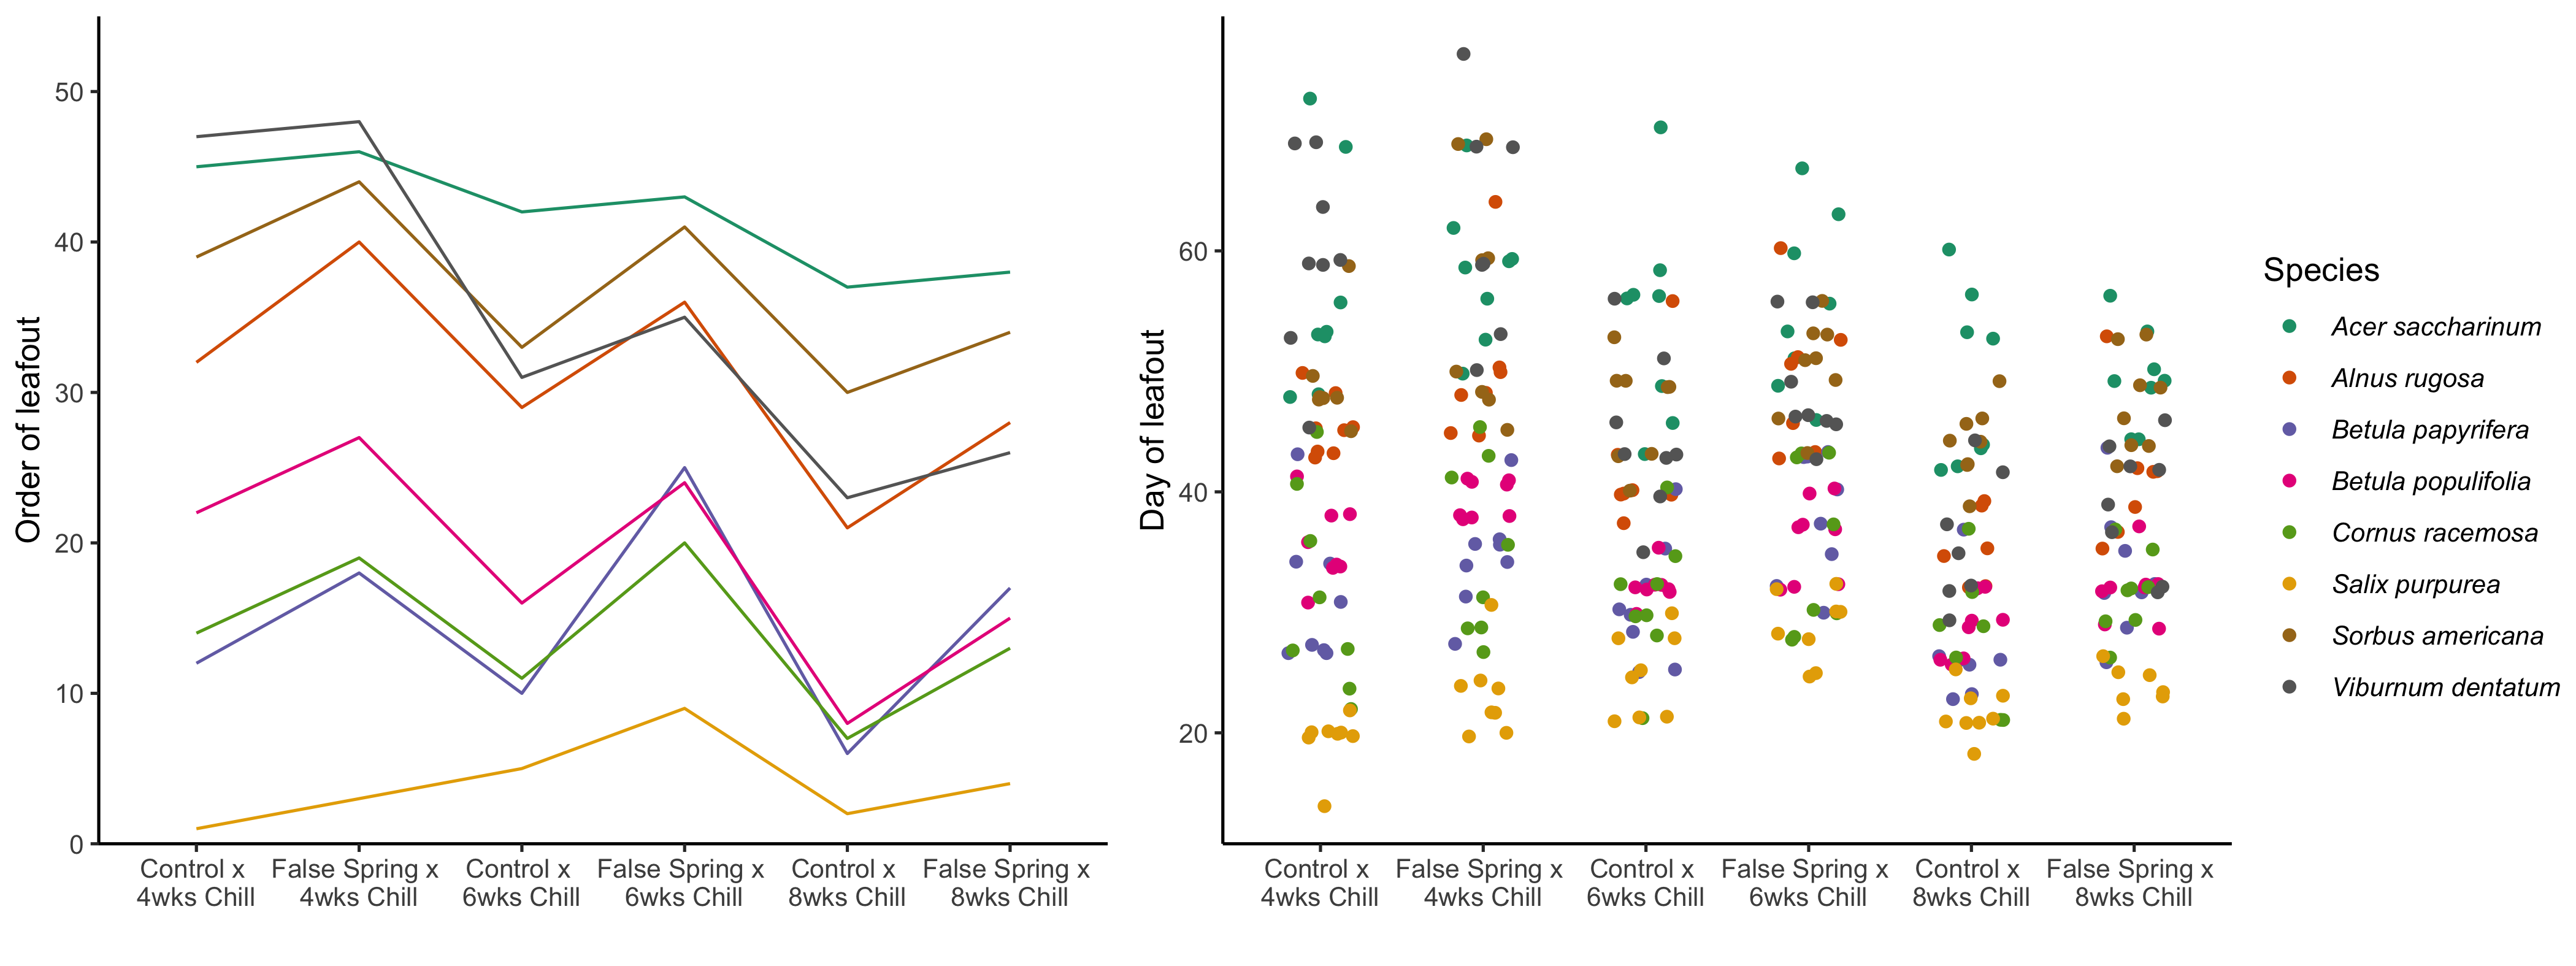
\includegraphics[width=18cm]{..//analyses/figures/leafout_orderandraw.png} 
  -\caption{Understanding rank order of leafout across all species using (a) mean trends and (b) raw estimates. }\label{fig:rank}
  -\end{center}
  -\end{figure}}
  
  {\begin{figure} [H]
  -\begin{center}
  -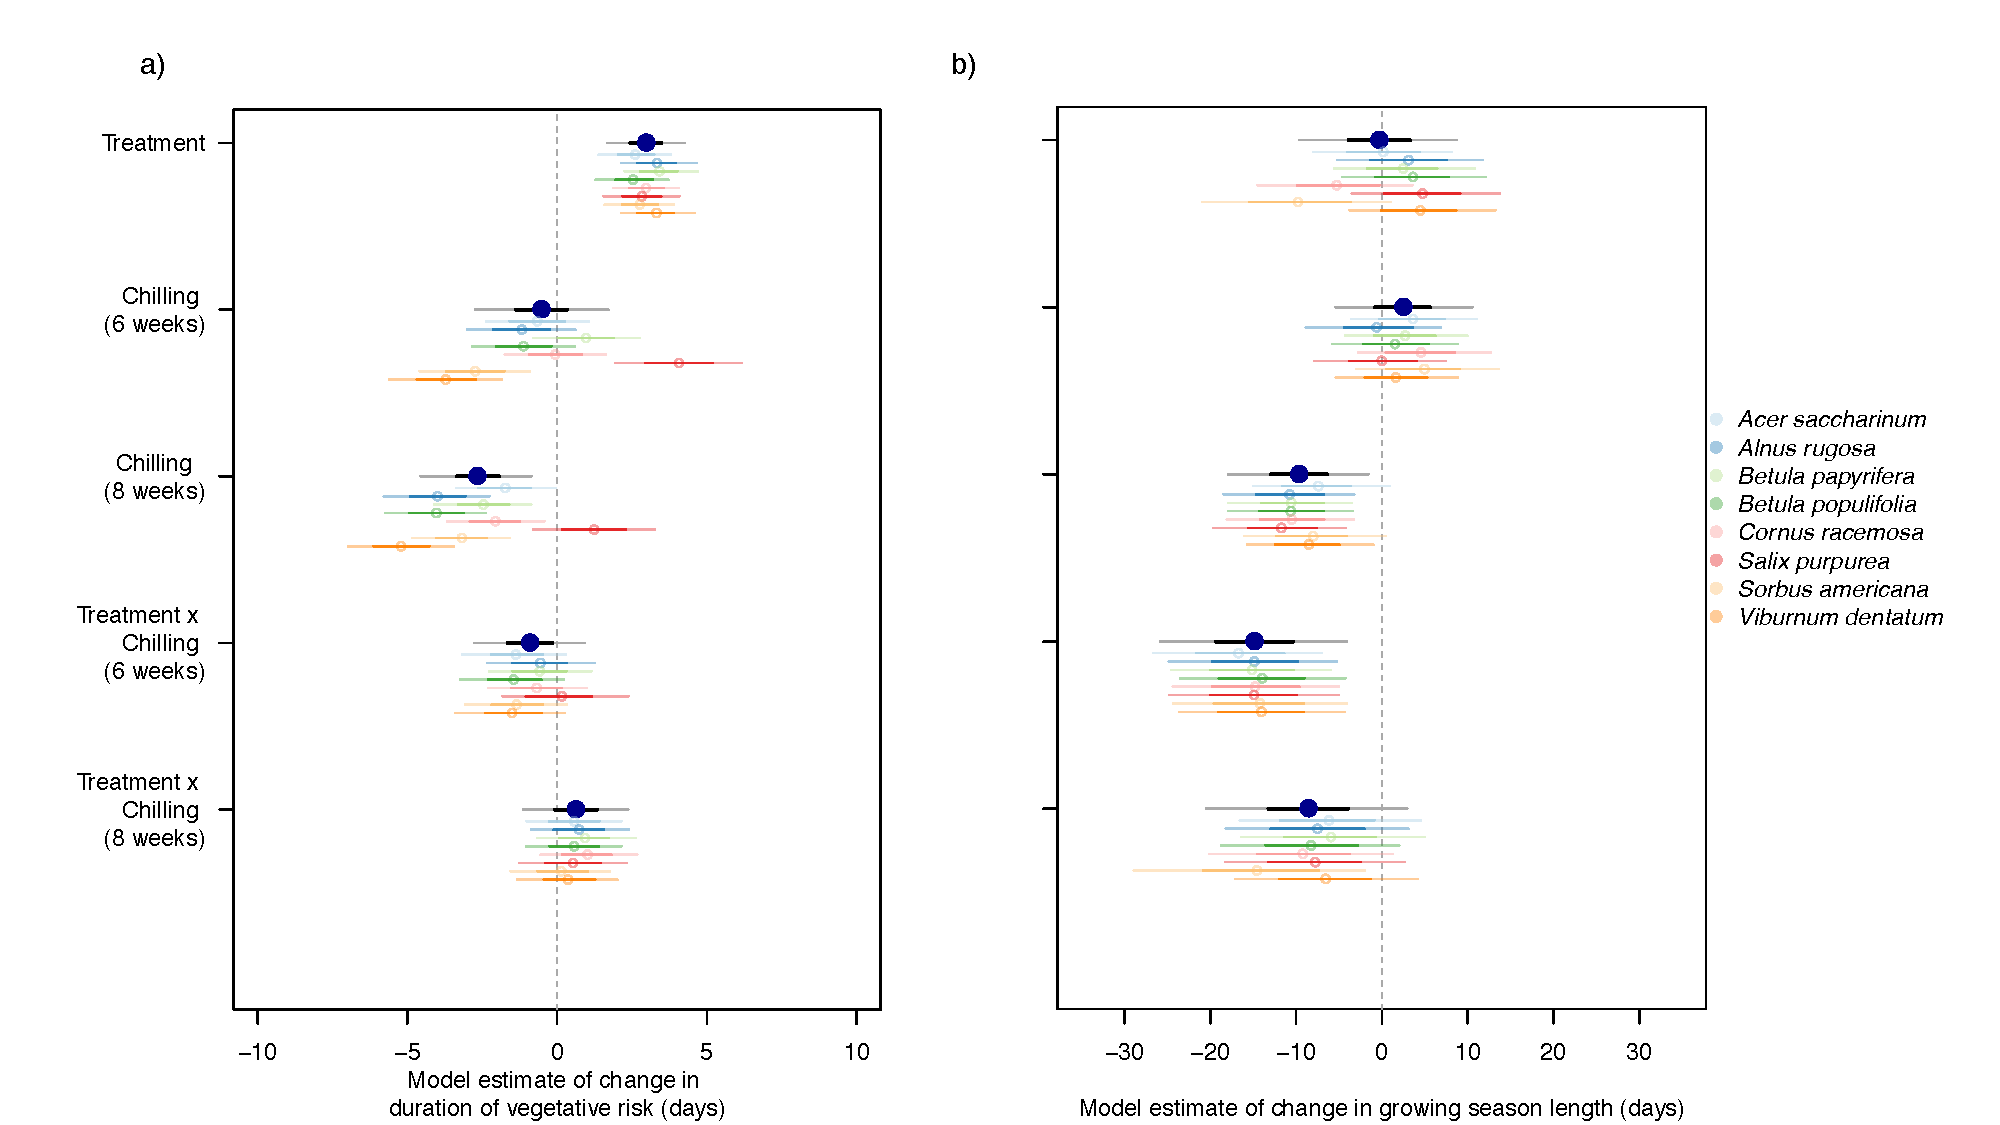
\includegraphics[width=18cm]{..//analyses/figures/mu_phen.pdf} 
  -\caption{Effects of false spring treatment, six weeks of chilling and eight weeks of chilling on a) duration of vegetative risk and b) growing season length. Dots and lines show means and 50\% uncertainty intervals.}\label{fig:muphen}
  -\end{center}
  -\end{figure}}
  
  {\begin{figure} [H]
  -\begin{center}
  -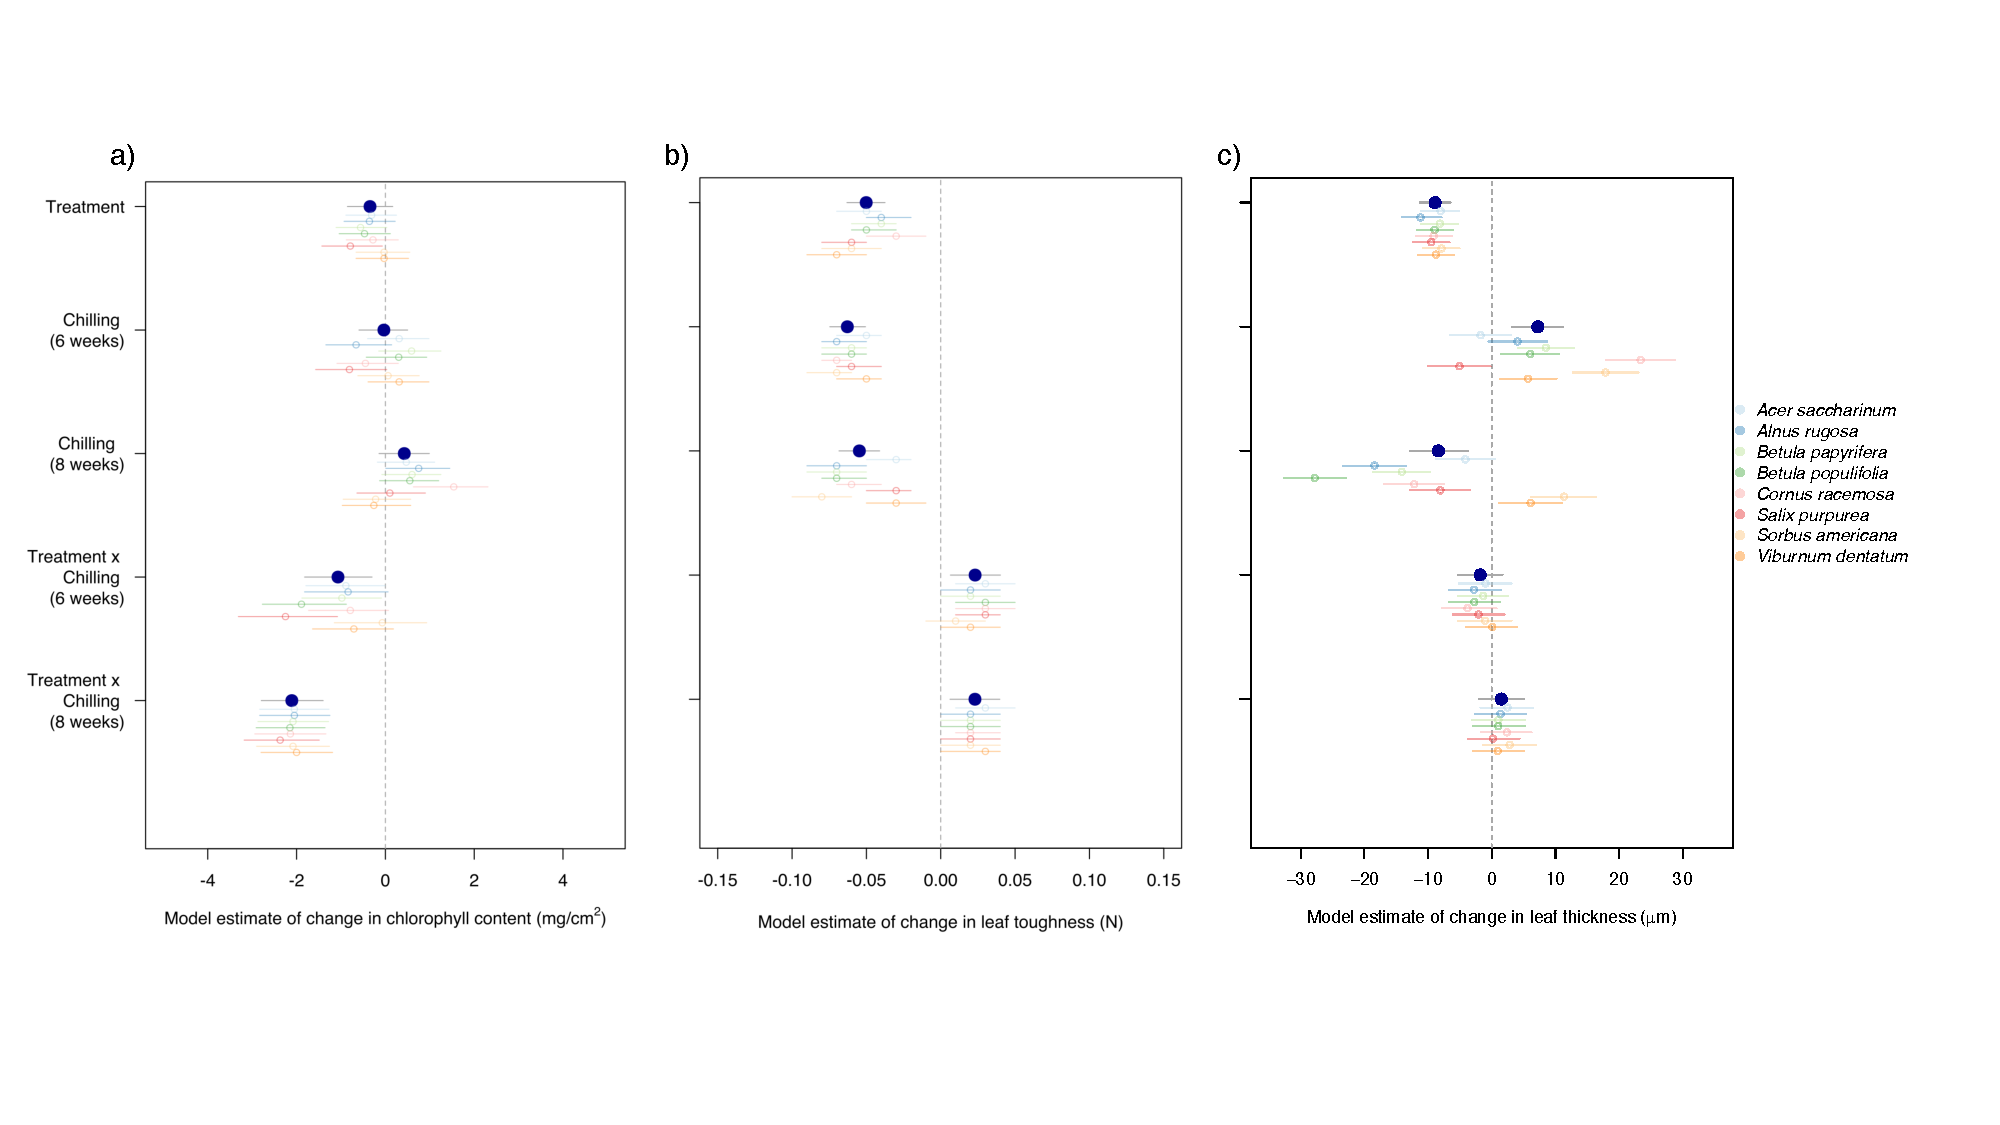
\includegraphics[width=18cm]{..//analyses/figures/mu_leaftraits.pdf} 
  -\caption{Effects of false spring treatment, six weeks of chilling and eight weeks of chilling on a) leaf toughness and b) leaf thickness. Dots and lines show means and 50\% uncertainty intervals. }\label{fig:muleaf}
  -\end{center}
  -\end{figure}}
  
  {\begin{figure} [H]
  -\begin{center}
  -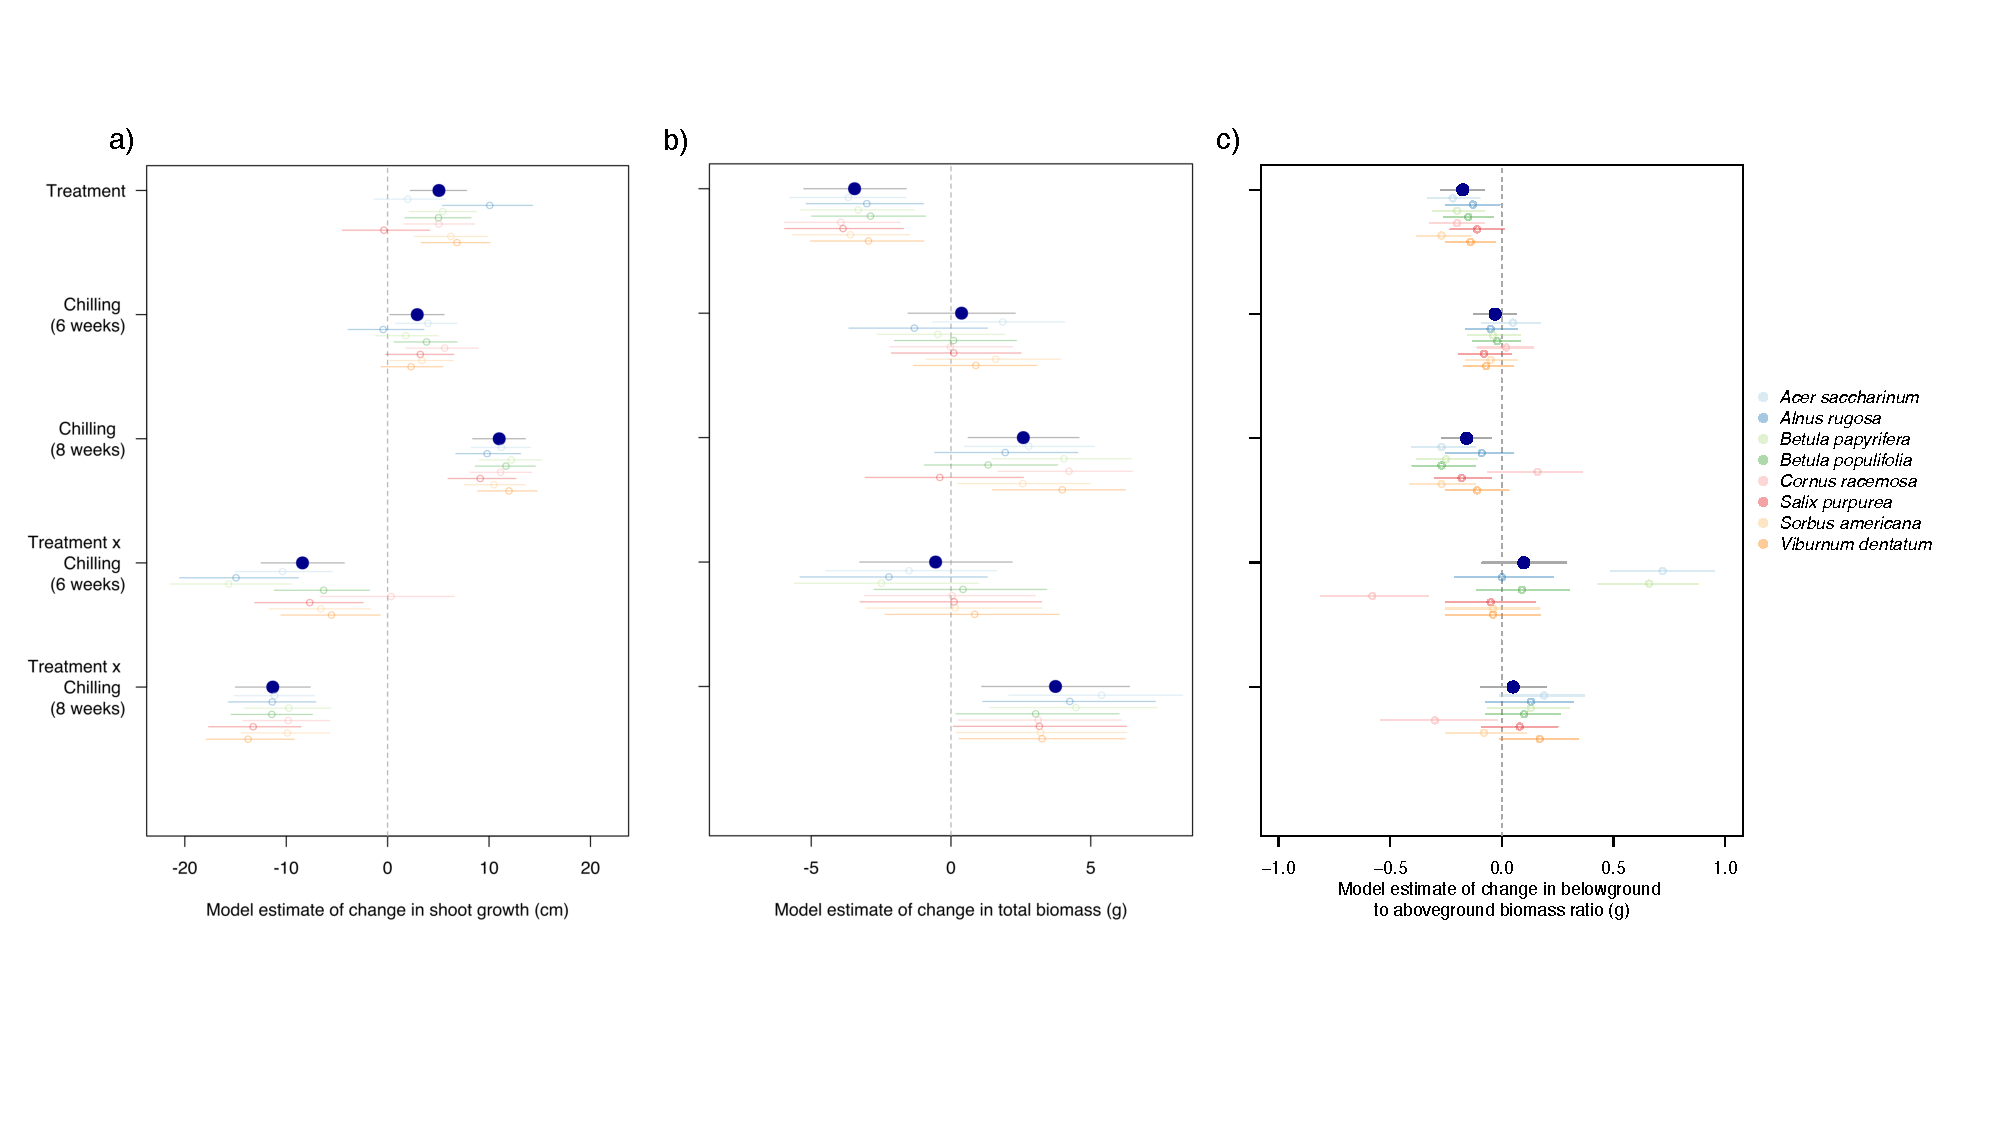
\includegraphics[width=18cm]{..//analyses/figures/mu_growth.pdf} 
  -\caption{Effects of false spring treatment, six weeks of chilling and eight weeks of chilling on a) shoot apical meristem damage and b) total biomass. Dots and lines show means and 50\% uncertainty intervals. }\label{fig:mugrowth}
  -\end{center}
  -\end{figure}}
  
  

\end{document}
